\section{Function Design}
\label{function-design}

During the brainstorm session many new functions were discovered.
As described in section \ref{brainstorm} each of them was assigned to a certain function group, \ie{} user, request, data, or publication.
With this knowledge the functions can be visualised with simple ordering based on the groups and prospective users as seen in appendix \ref{identified-functions}.
Each of the groups describe the management needs for the specific step in the research workflow (as described in section \ref{brainstorm} figure \ref{fig:workflow-after}).
When also considering the workflow the simple ordering can be fitted over it.
The result of this is shown in figure \ref{fig:functions-workflow} and will be described in the following paragraph.

\paragraph{Visualised}
In figure \ref{fig:functions-workflow} each of the functions belong to a certain actor (human or system), this is depicted by the colour of the actor block (light shade) and the corresponding colour of the function block (dark shade).
\allard{Think of some way to display without colours, not visible in black/white printing.}
The function groups are exempted from this rule as they only exist to give structure to the figure.
During the brainstorm session weight was given to the requirements, functions with less need for immediate implementation are displayed greyed-out (\ie{} change data, data curation, analyse, store outcomes).

When traversing the research workflow one should start from the {\tt user} block.
From here the {\tt register} function is the first step, the researcher registers as a user of the system.
After registering the account is send to the administrator user for {\tt approval}, hence the red colour for the function block.
Etcetera.
Each of the functions are mapped out according to the following story:

\begin{quotation}
	\noindent A researcher wants to investigate a certain hypothesis on the \project{} dataset.
	He or she needs to register an account with the system which is then checked and approved by the data manager.
	
	Next, the researcher formulates a data request on the system.
	From the data dictionary the researcher searches (filters) for the appropriate data items, names of data items are called headers.
	The researcher creates the request with the necessary information that the committee needs to base their decision on.
	The system provides feedback based on user entered or automatically detected keywords.
	Based on this feedback the researcher can edit the request or send it on for approval.
	The committee checks and approves the request.
	
	After approval the system creates a subset of \project{} data containing the requested data items.
	The researcher filters this subset and downloads a selection of the data.
	Another possible path is that the researcher prepares the data for analysis on the system and the outcomes are stored.
	
	To complete the request the researcher uploads his or her paper which is then again approved by the committee.
\end{quotation}

\begin{figure}[!htb]
	\centering
	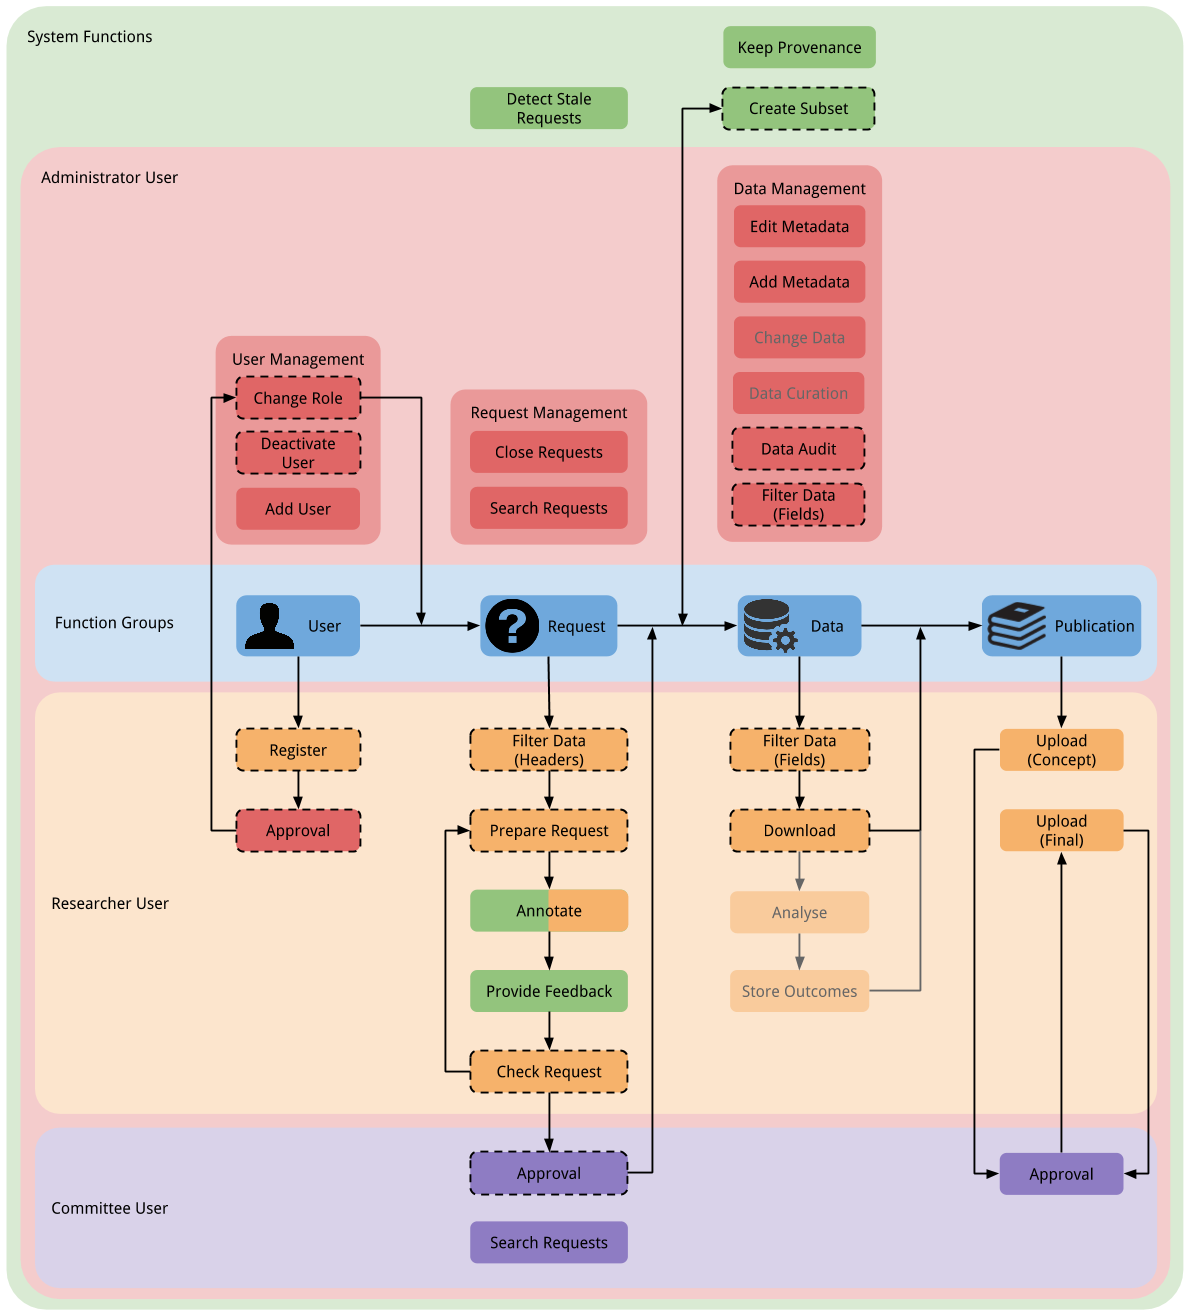
\includegraphics[width=1.0\linewidth]{images/functions-in-workflow}
	\caption{
		Mapping of functions according to function groups, actors, and research workflow.
		Vertical columns are used for function groups, colours are used for function to actor grouping, arrows are used to depict the workflow.
		Greyed-out functions are deemed less important, which was an outcome of the brainstorm session (see section \ref{brainstorm}).
	}
	\label{fig:functions-workflow}
\end{figure}